\subsection{Demand Calculation} \label{demandCalc}
%Janine

In Capitalism X, we assume that the demand for a product is based on customer satisfaction and the \textit{salesPrice}, the \textit{proxyPrice}, the \textit{totalProductQuality} and the \textit{proxyQuality}. 
The customer satisfaction influences the interest of the population in the respective products by shifting the price at which 100\% are interested.
 
The more satisfied customers are with the company, the more they are willing to pay for the same products. However, if customer satisfaction falls below 0.4, the \textit{overallAppeal} is influenced negatively. The following formula shows how the \textit{customerSatisfaction} affects the \textit{overallAppeal}.
\begin{equation}
\label{func:demandPrice}
\begin{aligned}
 oA_{demand} = oA \cdot (0.8 + cS \cdot 0.4)
\end{aligned}
\end{equation}

In order to make the demand of CapitalismX clients more similar to that of a real market, the demand curve is not linear. 
% explain wy the curve is lie this, example values -> oA = 2 dPC = ....

The \textit{demandPercentage} (\gls{dPC}) is calculated by using the \textit{overallAppeal} as input for the following function. 
\begin{equation}
\label{func:demandPercentage}
\begin{aligned}
% dPC(oA_{demand}) = tanh(oA_{demand}/2)
dPC(
\end{aligned}
\end{equation}

Figure \ref{demand_function} shows the course of the \textit{demandFunction}. The x-axis corresponds to the \textit{overallAppeal} of a product and the y-axis to the percentage interest of the population, the \textit{demandPercentage}. 

\begin{figure}[h]
\centering
\begin{tikzpicture}
\begin{axis}[
    xmin=-0.1, xmax=4,
    ymin=-0,1, ymax=1.2,
    axis lines=center,
    axis on top=true,
    domain=-2.5:4,
    ylabel=$dPC$,
    xlabel=$oA$,
    ]

    \addplot [mark=none,draw=red,ultra thick] {tanh(\x/2)};
    \node [right, black] at (axis cs: 1,0.3) {$y = \tanh x/2$};
    \draw [blue, dotted, thick] (axis cs:+4,+1)-- (axis cs:0,+1);
\end{axis}
\end{tikzpicture}
	\caption{demandPercentage function}
	\label{demand_function}
\end{figure}

The \textit{demandAmount} (\gls{dA}) for a product is finally calculated by combining the demand in percent with the \textit{gamePopulation} (\gls{gP}). This approach enables the total demand to be higher than the actual quantity of products offered.
\begin{equation}
\label{func:demandAmount}
dA = dPC \cdot gP    
\end{equation}

After calculating the $demandAmount$ for the entire product lifecycle we have to calculate the demand for a single day.

Since we don't sell the total demand at once but distributed over a longer period of time after the product has launched we need to specify a function which calculates the $demandAmount$ for a single day. For a product $p$ we can calculate the $daysSinceLaunch$ (\gls{dSL}) as follows:
\begin{equation}
	daysSinceLaunch_p = t_d -launchDay_{p}
\end{equation}
As the following calculations are performed per product we will implicitly assume but omit the $p$ index.
We can calculate the periodicDemandAmount \gls{pDA} for each day using the \gls{dSL}):
\begin{equation}
\begin{aligned}
pDA(dA, \gls{dSL}) = dA \cdot 0.002\cdot (\frac{-tanh(0.01 \cdot dSL-3)}{2} + 0.5)
\end{aligned}
\end{equation}

%figure: 0.002 *(−tanh(0.01* x−3)/2+ 0.5)
\begin{figure}[h]
\centering
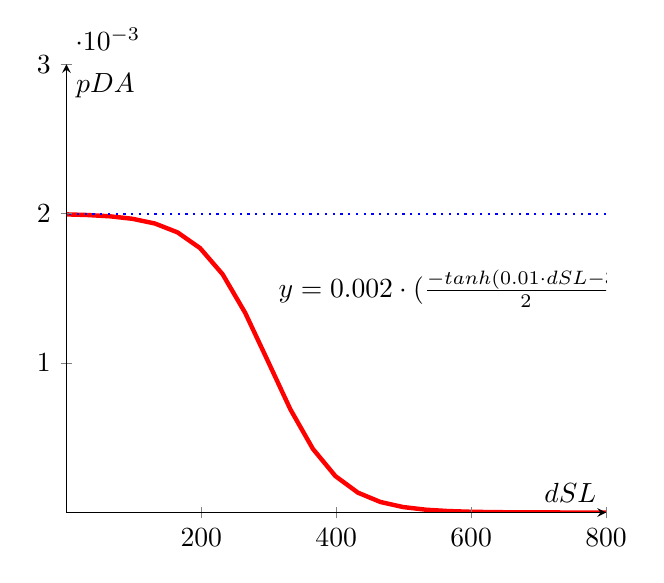
\begin{tikzpicture}
\begin{axis}[
    xmin= 0, xmax=800,
    ymin= 0, ymax=0.003,
    axis lines=center,
    axis on top=true,
    domain=-2.5:800,
    ylabel=$pDA$,
    xlabel=$dSL$,
    ]
    % This somehow causes a timeout
    %\addplot [mark=none,draw=red,ultra thick] {0.002*(-\tanh(0.01 * \x - 3)/2+0.5)};
    \addplot [mark=none,draw=red,ultra thick] {
    	0.002*(-tanh(0.01 * \x - 3)/2 + 0.5)
    };
    \draw [blue, dotted, thick] (axis cs:+800,+0.002)-- (axis cs:0,+0.002);
    \node [right, black] at (axis cs: 300,0.0015) {$y = 0.002 \cdot (\frac{-tanh(0.01 \cdot dSL-3)}{2}) + 0.5)$};
    
\end{axis}
\end{tikzpicture}
	\caption{periodicDemandAmount function}
	\label{periodicDemandAmount_function}
\end{figure}


This function covers the entire demand over a longer period of time as
\begin{equation}
	\int_{0}^{\infty} 0.002 \cdot (\frac{-tanh(0.01 \cdot dSL-3)}{2} + 0.5)\; \mathrm{d} dSL = 1  
\end{equation}

The quantity actually sold by the company, so-called \textit{salesFigures} per product (\gls{sFP}), depends on whether the actual demand exceeds the \textit{numberOfferedProducts} (\gls{nOP}) or not.
\begin{equation}
\label{func:salesFigure}
\begin{aligned}
sFP = 
\begin{cases}
     nOP & \text{if} \; pDA > nOP\\
     pDA & \text{otherwise} \\
\end{cases}
\end{aligned}
\end{equation}

For the calculation of the \textit{marketShare} (\gls{mS}) it is assumed that the proportion of the population who would have liked to buy a product but went away empty-handed buys its product from a competitor. The company's \textit{totalMarketShare} (\gls{tMS}) is calculated using the sum of the sales figures of the single products and the sum of the demands for them. Following formulas show the calculation of the market share of a product and the total market share of the company. 
\begin{equation}
\label{func:marketShare}
\begin{aligned}
% I'd rather use:
%MS = \frac{sFP}{population} \\
mS = \frac{sFP}{dA} \\
tMS = \frac{\sum_{p \in P}(sFP)}{\sum(dA)}  
\end{aligned}
\end{equation}

